\section{Platform Description}

In this section, we present an overview of \meddle.\footnote{\meddle is currently in private beta with deployments in the US, France and China. User's sign-up for an IRB approved study through \url{http://meddle.mobi}. We will make the \meddle software publicly available.} 
The goal of \meddle is straightforward: \emph{we seek to monitor and control a mobile device's Internet traffic with the aim to diagnose the behavior of mobile apps, OS services, and traffic interference from ISPs}. 
While previous work has accomplished this for a limited set of devices or networks, we seek to avoid such limitations. 
Indeed, there exists a trade-off between a practical user-friendly solution and a solution that offers a fine-grained control over mobile devices and the traffic they generate.
Unlike existing approaches, we take the direction for a practical and user-friendly solution and test the limits of its usefulness.
Specifically, we relinquish OS-level controls to focus on the Internet traffic generated by mobile devices and try to use this perspective to diagnose mobile apps, OS services, and the ISPs that serve these devices.
\tbd{Do we pitch user friendly or research friendly?}

The following sub-goals governed the \meddle's design.
\begin{packedenumerate}
\item \emph{Agnostic to OS, ISP, access technology, and applications.}.
The research work that comes out must not be limited to specific OS, ISP, or device manufacturer, or set of applications.
In particular, \meddle avoids the need to develop OS-specific applications, or to warranty void the device. 
\meddle must also be able to monitor and interpose on traffic without explicit support from ISPs and cellular providers, and should work regardless of the access technology used by the device (\wifi, GSM, CDMA, UMTS, LTE, \etc.). 
\item \emph{Always-On.}
Once enabled by the user, \meddle must automatically support switching between networks or when device returns from being idle.
Specifically, it must not demand inputs from end-users on network state changes. 
\item \emph{On-demand}.
Users must be able to enable and disable service on-demand.
This is important to ensure that users can easily opt-in to the system when they want to use a feature offered by \meddle and at the same time users can easily disable the system when they encounter some problems with \meddle. 
%It must be easy to fallback to the original state.
\item \emph{Deployable.}
\meddle must be easy to install, use, and configure.
\meddle should be equally feasible to deploy on a single machine, such as a home-gateway, or using a collection of VMs in a hosted/cloud deployment. 
This is important to support a large user-base.
\item \emph{Scalable.}
To ensure that research results have statistical significance, \meddle must be able to scale to support a large user-base.
\item \emph{Traffic Interposition.} 
We want to not only monitor, but also possibly modify data packets in order to experiment. 
This makes \meddle both a passive monitoring and an experimental platform. 
\item \emph{Encryption agnostic.} 
\tbd{Interpose on encrypted traffic?}
Achieve visibility of both encrypted and plaintext traffic.
\end{packedenumerate} 
Each of these sub-goals is inherently aimed at making \meddle work in unison with existing tools for mobile diagnosis. 
In the rest of this section, we detail \meddle's design, then we discuss \meddle's feasibility and limitations.

\subsection{Design}

\meddle attains its goals by exploiting the observation that nearly all devices support network traffic indirection via virtual private networks (VPNs) and HTTP proxies. 
This network perspective offered by traffic redirection is promising because mobile devices are increasingly becoming the primary gateway to access Internet based services~\cite{ict:facts}. 
This perspective becomes even more important because a large number of free applications use Internet connectivity with the sole purpose of serving advertisements that make-up for their costs~\cite{pathak:eprof,vallina-rodriguez:bfc}.

\begin{figure}[h]
\centering
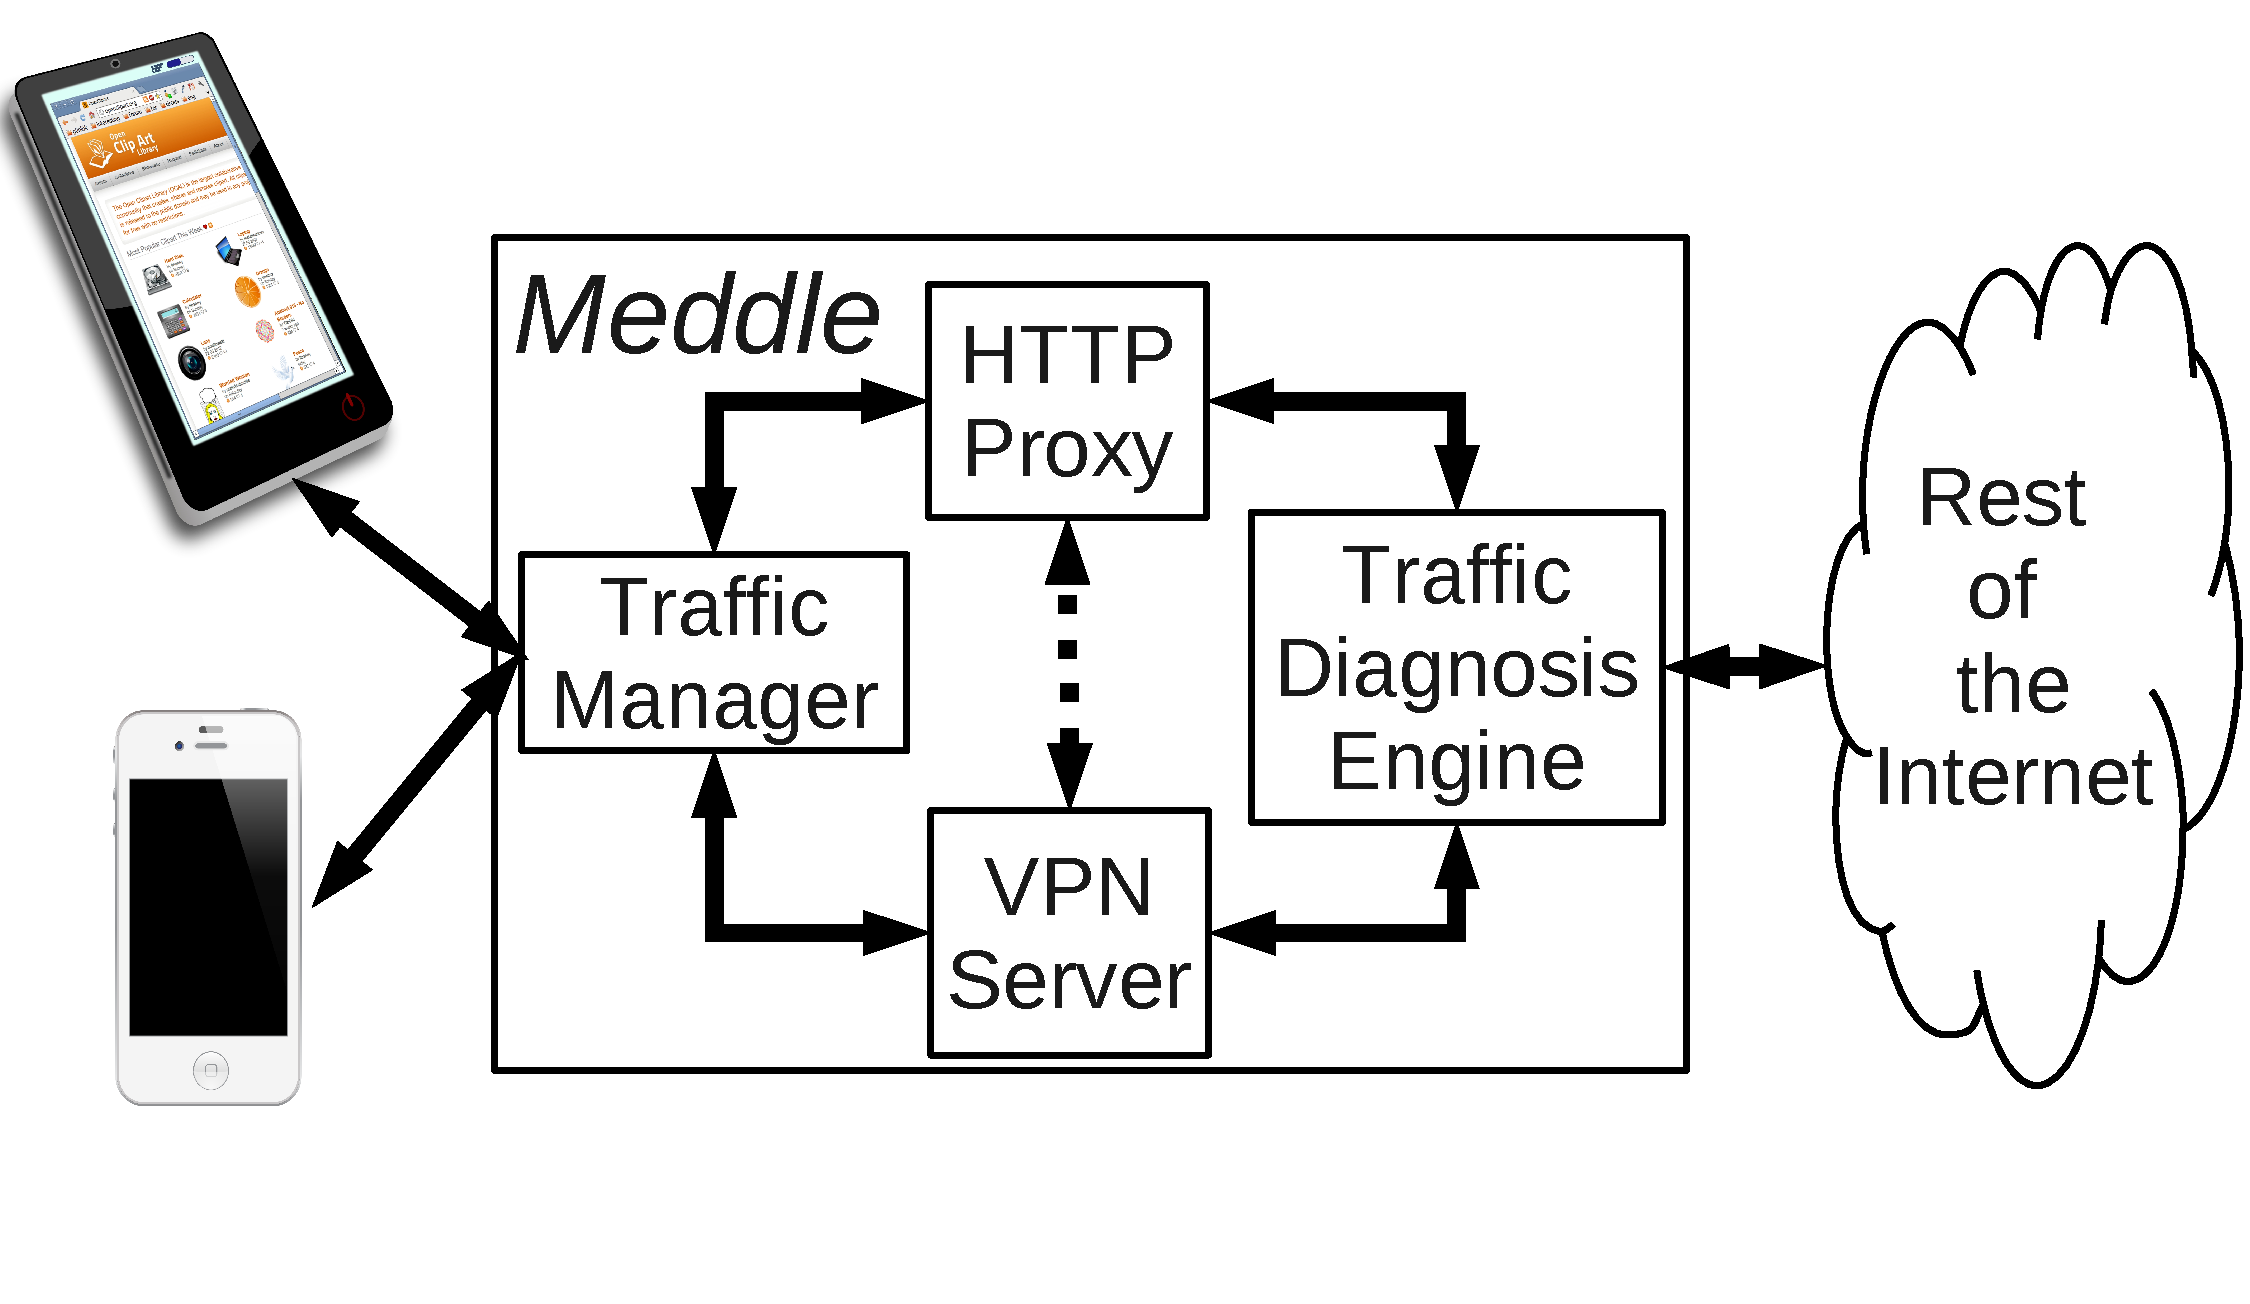
\includegraphics[width=\columnwidth]{figures/Meddle-Design.pdf}
\caption{Traffic diagnosis using VPN and HTTP proxy based traffic redirection.}
\label{fig:architecture}
\end{figure}
As depicted in Figure~\ref{fig:architecture}, \meddle relies on a combination of VPN and HTTP based proxies to diagnose traffic from mobile apps and OS services, and to identify ISP interference.
\meddle uses HTTP proxies, that exchange traffic in the clear, to identify possible ISP interference with HTTP traffic. 
\meddle uses VPNs to address potential ISP interference, and to diagnose the traffic naturally generated by the mobile apps and OS services.

\meddle's traffic manager determines the flow of the packet, through a combination of VPN and HTTP proxies, before the packet enters the traffic diagnosis engine. 
On this engine, we deploy a variety of diagnosis tools such as bro. 
\tbd{Here it must be highlighted that \meddle allows the integration of the existing tools to offer a single platform that can be used for mobile traffic diagnosis. Though simple, it brings with it a power that previously required warranty voiding of devices and ... The novelty lies in exploiting existing features to come up with a feasible user friendly platform}



VPNs are supported by most mobile OSes\footnote{Android, BlackBerry, and iOS all support VPNs natively, representing more than 86\% of the mobile device market\cite{gartner-phone-share}.} and carriers to satisfy their enterprise clients. 
Thus \meddle leverages on VPNs for being agnostic to mobile OSes, ISPs, access technologies, and applications used by the mobile device.
\tbd{what about other goals.. I do not want to put a see section .. here.}

%\subsubsection{Architecture}

\meddle uses VPNs as a portable mechanism to tunnel traffic from mobile devices to a machine outside of the carrier's network for the purpose of analysis and interposition.
\meddle uses the Squid~\cite{squid} HTTP proxy for two purposes: 1) to monitor the SSL traffic using SSL bumping~\cite{sslbump} which is essentially a man-in-the-middle operation, and 2) inject javascript code inspired by tripwires~\cite{tripwires} to identify ISP interference.

\meddle currently offers the following capabilities to diagnose mobile Internet traffic
\begin{packedenumerate}
\item Passive monitoring to characterize the network behavior of application and OS services. 
\item Enhanced passive monitoring to analyze SSL traffic.
\item Analysis of ISP interference.
\item Filtering privacy invasive traffic. 
\end{packedenumerate}

\subsubsection{VPN Configuration to Monitor and Interpose on all Internet Traffic}
\label{sec:VPN Configuration}

\meddle exploits the out-of-the-box VPN support by mobile devices, a feature provided to satisfy enterprise clients. 
Manually configuring a VPN generally requires filling out five fields on an Android phone, and the VPN configuration can be distributed using a single file on iOS. 
These configurations are primarily required to drive the key exchange algorithms required to establish the VPN tunnels. 

\noindent\textbf{iPhone support.} 
All iOS devices (version 3.0 and above) support \textit{VPN On-Demand}, which forces traffic for a specified set of domains to use VPN tunnels. 
This feature is originally intended to allow enterprises to ensure their employees' devices always establish a VPN connection before contacting a specified set of domains. 
To ensure all possible destinations match this list, we exploit the fact that iOS uses suffix matching to determine which connections should be tunneled; accordingly, we specified the domain list as the set of alphanumeric characters (a-z, 0-9, one character per domain). 
To setup this configuration, users need to install a single file, a step that needs to be performed only once. 

\noindent\textbf{Android support.} As of Android 4.2, Android supports ``always on'' VPN connections that ensure all traffic is always tunneled.
For Android version 4.0 and above there is an app API that allows apps to manage VPN tunnels. 
We use this API in the StrongSwan implementation of a VPN client~\cite{strongswanclient} that ensures re-establishment of VPN tunnels on network state changes (\eg, when a device switches from cellular to \wifi).
\meddle is thus supports devices running Android version 4.0 and above.

\noindent\textbf{Server-side implementation.} 
\meddle uses the free and open-source Strongswan~\cite{strongswan} to manage the VPN tunnels on its servers. 

\subsubsection{Configuration to Intercept SSL Traffic}

We now describe we describe how \meddle allows us to analyze the contents of SSL flows generated by mobile devices.
First, we note that \meddle's VPN server, like all VPN servers, can be configured to use self-generated root certificate used to sign all subsequent certificates issued to participating mobile devices. 
This allows us to perform SSL traffic decryption using the Squid proxy's SSL bumping~\cite{sslbump} feature, which is essentially a man-in-the-middle operation on the secure connection.
When the mobile device connects to a services supporting SSL, the proxy masquerades as the service using a forged certificate signed with the \meddle root certificate. 
Then the proxy establishes an SSL connection with the intended target, impersonating a mobile device. 
Using the traffic captured on \meddle and the private key generated by the squid proxy to communicate with the mobile device, we can decrypt all SSL traffic.
We note that when traffic is not encrypted using SSL, the proxy simply forwards traffic. 

This approach fails for apps that do not trust certificates signed by unknown root authorities. 
For example, in our controlled experiments we observed that Firefox prevents SSL bumping by validating root certificates, while the Google Chrome, Safari, Facebook, and Google+ apps, as well as the default mail clients and advertisement services, do not check the validity of the root certificate. 
This enables our approach to provide visibility into secure channels established with a wide range of popular apps. 


\subsubsection{DNS based packet filter}

We use \meddle's capability to interpose on traffic to block leaks of personals identifiable information (PII).
As described in Section~\ref{sec:}, we use \meddle to create a database of sites that leak PII information. 
This database is also augmented using results of existing studies~\cite{vallina-rodriguez:bfc, hornyack:appfence,pathak:eprof}.
\meddle relies on this database to filter the DNS responses. 
Using this simple technique, \meddle has the potential to complete the loop of identifying problems and providing solutions to fix them. 

\subsection{VPN Overheads}

\noindent\textbf{Increase in Network Latency.}
We measured 50 VPN-connection establishment times  on both iOS (iPhone 5 / iOS 6.1) and Android (Galaxy Nexus /
Android 4.2), for \wifi{} and cellular connections. 
The \meddle server was running on a university network. 
For Android (using IKEv2), the maximum establishment time was 0.81 seconds on \wifi{} and 1.59 seconds on cellular. 
For iOS (using IKEv1), the connection takes longer due to the older protocol version: we observe a maximum of 2 seconds on \wifi{} and 2.18 seconds on cellular. 
Because each VPN session supports many flows, the amortized cost of connecting is  small. 
\tbd{Cite results from latency to home gateways based on DSL results in PAM and IMC.}
\tbd{Address comments in conext review on latency}

\noindent\textbf{Increase in Power Consumption.}
Mobile devices expend additional power to establish, maintain and encrypt data for a VPN tunnel. 
To evaluate the impact on battery, we used a power meter to measure the draw from a Galaxy Nexus running Android 4.2. 
We run 10-minute experiments with and without the VPN enabled. 
For each experiment, we used an activity script that included Web and map searches, Facebook interaction, e-mail and video
streaming. 
The VPN leads to a 10\% power overhead. \tbd{min, max, median for results given by dave}. 
For iOS devices, we relied on the battery readings provided by iOS because we cannot attach a power meter directly to the battery.
We again found an approximately 10\% power overhead of using VPNs when we drained a fully charged battery while performing the operations performed during the tests for Android devices.  

%\item 
\noindent\textbf{Increase in Traffic Volume.}
\meddle relies on IPsec for datagram encryption, thus there is an encapsulation overhead for each tunneled packet. 
To evaluate this overhead, we use 30 days of data from 25 devices that to compare encapsulated and raw packet sizes. 
We observe a maximum encapsulation overhead of 12.8\% (average approximately 10\%). 
Within the scope of the traffic monitoring experiments performed with \meddle, the impact of this overhead is negligible. 
However, in case of experiments with a limited cellular data plan, this overhead must be taken into account
%\end{packedenumerate}

\subsection{Limitations}

\noindent\textbf{At most one VPN tunnel.}
Currently iOS and Android support exactly one VPN connection at a time. 
This allows \meddle to measure traffic over either \wifi or cellular interfaces, but not both at once.
The vast majority of traffic uses only one of these interfaces, and VPNs can be used to tunnel that traffic
\tbd{MPTCP on iOS 7??}

\noindent\textbf{Proxy location.} 
When traffic traverses \meddle, destinations will see the \meddle box address, not the device IP, as the source. 
This might impact services  that customize (or block access to) content according to IP address (e.g., in case of localization). 
A solution to this problem is to use a \meddle{} instance with an appropriate IP address

\noindent\textbf{ISP support.}
Some ISPs block VPN traffic, which prevents access to our current \meddle implementation. 
We note that few ISPs block VPN traffic, and there is an incentive not to block VPN traffic to support enterprise clients.

\noindent\textbf{IPv6.}
\meddle{} cannot be currently used on networks using IPv6 because IPv6 is not fully supported by mobile devices. 
Indeed, we observe that though iOS and Android support IPv6 they currently do not support IPv6 traffic through VPN tunnels


%\noindent\item \textbf{Wi-Fi Gateways powered by Cellular Modems.}


\subsection{Costs}

\noindent\textbf{Deployment and Running Costs}

\noindent\textbf{Trust Provider}

\subsection{Incentive for Deployment}

\noindent \textbf{Deploy on Home Gateway.}
This is why we need the single machine constraint. 

\noindent \textbf{Packet Filtering.}
Custom ad blocks. Protect against data leaks. 

\noindent \textbf{User Interface to Packet Filtering.}

\noindent \textbf{Security from untrusted Wi-Fi APs.}

%\noindent \textbf{Modular Architecture for Offloading Activities.}



%%% Local Variables: 
%%% mode: latex
%%% TeX-master: "meddle-main"
%%% End: 
